\documentclass{article}
\usepackage{graphicx} % Required for inserting images
\usepackage[UTF8]{ctex}
\usepackage{geometry}
\usepackage{listings}

\graphicspath{{pics/}}
\newgeometry{left=2cm, right=2cm, top=2cm, bottom=2cm}

\title{ 编译(H)期末报告 }
\author{ 张鑫 21307130295}

\begin{document}

\maketitle

\section{Introduction}
复旦大学编译(H)课程以Fudan MiniJava(MiniJava的一个子集,一种类java语法的简单语言)为源语言,详细阐述了一个最基本的、完整的编译器的整个过程与结构,并要求学生利用所学知识,实现一个Fudan MiniJava的编译器,最终生成arm上的目标汇编代码并用qemu模拟运行,检验正确性。

本报告旨在总结本人在课程中的所学所获,主要对整个编译流程及其对应的代码实现进行阐述,以便未学习本课程的计算机学生或感兴趣人士,能够对较为容易地理解我的编译器的代码实现。

本课程和报告所涉及的编译器采用前后端分离的设计,使用Tiger IR+和LLVMIR作为中间表示(intermediate representation)。前端过程主要包括Parsing、Type Checking、Translation to IR和Canonicalization;后端过程主要包括LLVM Instruction selection、Liveness analysis、Static Single Assignment、RPi Instruction selection和Register allocation。

接下来,本报告将详细阐述前端流程和后端流程的每一个阶段在我的编译器中的具体实现方式。在Section “Frontend”中我将详细阐述前端,在Section “Backend”中我将详细阐述后端,最后简单介绍我实现的编译器的构建和使用方式,并总结我一学期以来的所学所获。

在正式开始之前,我将提供一个样例.fmj程序,以之为案例详细解释每一个阶段到底做了什么工作。完整程序见/docs/example/example\_in\_report.fmj

\section{Frontend}
\subsection{Parsing}
Parsing是整个编译的第一阶段,其目的是将源程序的字符串形式的代码去除注释后,转换为具有结构、语义等信息的抽象语法树(Abstract Syntax Tree,简记为AST)。

在我的实现中主要分为词法分析和语法分析。其中词法分析通过Lex快速生成词法分析器,将字符串形式的代码转换为一系列合法的terminal,在这个过程中,如果遇到不合法的字符串(例如不合法的标识符:0xaw)会产生由词法分析错误导致的“Syntax Error”;语法分析通过Yacc快速生成语法分析器,语法分析器接收由词法分析器输出的一系列terminal,根据事先用CFG(Context-Free Grammar)定义好的语法规则进行派生,不断重复进行“匹配——动作”。在每一条语法规则的动作中,调用对应的AST节点的初始化函数,返回这个AST节点,并将之与派生出的non-terminal符号所关联,以便递归使用。例如样例程序中的length(d.c),根据我们的语法规则,d.c会被派生为一个EXP,并且将它匹配-动作过程中得到的AST节点(记为node\_a)与之绑定。因此length(d.c)会得到length(EXP),又对应了另一条语法规则,因此又可以返回新的AST节点A\_LengthExp(pos, node\_a),如此反复,我们最终会得到AST的根节点A\_Prog。

在Parsing的语法分析阶段,我实现了如下3种错误报告、处理和恢复:
\begin{itemize}
    \item \textbf{缺失的分号}:例如当样例程序中第9行的分号去除,则编译器会输出错误提示信息:“Line\_9: ';' expected”,并且跳过到下一个合法处,继续进行后续的语法分析。具体做法是定义了一个non-terminal符号:CHECK\_SEMI,用它替换每一条语法中末尾出现的分号,则根据它的CFG语法规则,当缺少分号时,会跳到最近的“\}”或者“;”,但是为了不破坏“\}”与之前的匹配,需要自行在输入流中加入一个“\}”,使用定义在src/lib/frontend/lexer.lex文件末尾的add\_char函数完成此功能,调用lex的unput函数实现。将分号替换为CHECK\_SEMI后,需要进行错误报告和恢复,使用如上图自定义的函数check\_semi,根据CHECK\_SEMI返回的值来判断是否发生缺失分号,并报告错误行数最后调用yyerrok恢复正常parsing。

    \item \textbf{缺失的成对小括号}:处理逻辑与“缺失的分号”相同,都是通过新定义一个特殊的non-termin符号:CHECK\_PARENT和其对应的检查函数check\_parentheses实现。
    
    \item \textbf{形参缺失类型定义}:处理方式为,在缺失类型定义的地方设置error的检查,忽略后续所有的形参声明,一直跳过到形参定义的结束标志:“)”。

\end{itemize}

完成Parsing后我们得到一颗完整的抽象语法树,其根节点即main.c中的“A\_prog root;”。将其打印输出得到可视化的抽象语法树结构,结果见/docs/example/example\_in\_report.2.ast文件。

\subsection{Type Checking}
Type Checking是针对Parsing阶段得到的AST进行类型检查,这是因为一个程序可能符合语法,但是符合语法的语句不一定有实际意义。例如样例程序中,变量b是一个class类型的变量,如果我们对它赋值为0,或者定义了一个未定义的类为类型的变量等等,都是不允许出现的情况。我们希望在类型检查阶段对所有的表达式的类型进行严格的检查,只允许int和float的隐式转换,子类和父类的upcast,以减少“即使符合语法规范,但是编译出的程序无法正常运行”的情况。并且在检查到错误的类型时输出相应的提示信息和出现的位置信息,例如上述例子,输出:“(line:7 col:5) Assignment between incompatible types.”。

我的编译器中,该过程实现在文件src/lib/frontend/semant.c中,入口为:

    \begin{lstlisting}
    T_funcDeclList transA_Prog(FILE *out, A_prog p, int arch_size);
    \end{lstlisting}

其中out是输出错误信息的文件对象,p是一个AST的根节点;arch\_size是所使用的架构所使用的字大小,为8表示64位,为4表示32位,对本阶段而言可暂时忽略。该函数主要进行Type Checking的初始化,然后调用对应的函数,分别对所有类定义和主方法进行类型检查。

\subsubsection{类的检查过程}
类检查的入口函数为transA\_Classes。

首先调用build\_cenv函数构建类环境。我的类环境是一系列表,但对于类型检查阶段而言,只涉及到表CENV,记录了“类名-->ClassEntry”的映射。每一个ClassEntry包含了类定义的ast节点、父类名、类继承检查状态、变量环境(venv)和方法环境(menv)。build\_cenv遍历每一个类,首先检查是否重定义,然后调用transA\_VarDecList函数进行变量的类型检查,构建venv;调用build\_menv构建menv,然后插入一条“类名-->ClassEntry”到表CENV中。需要注意的是,在检查类变量的类型时,如果碰到变量的类型是一个类,暂时跳过它,因为可能它的类还没有被加入到CENV,在后续检查。

然后调用check\_inheritance进行类继承的检查,以每一个类继承检查状态为E\_transInit的类为入口,递归检查它的父类是否存在,并在继承父类的方法和变量的过程中,检查是否存在变量重定义和方法重写的正确性。处理继承父类的变量的函数为inherit\_vars,处理继承父类方法的变量为inherit\_mtds。

以样例程序为例,构建完类环境CENV之后,我们得到如下表和数据结构:
\begin{figure*}[h]
  \centering
  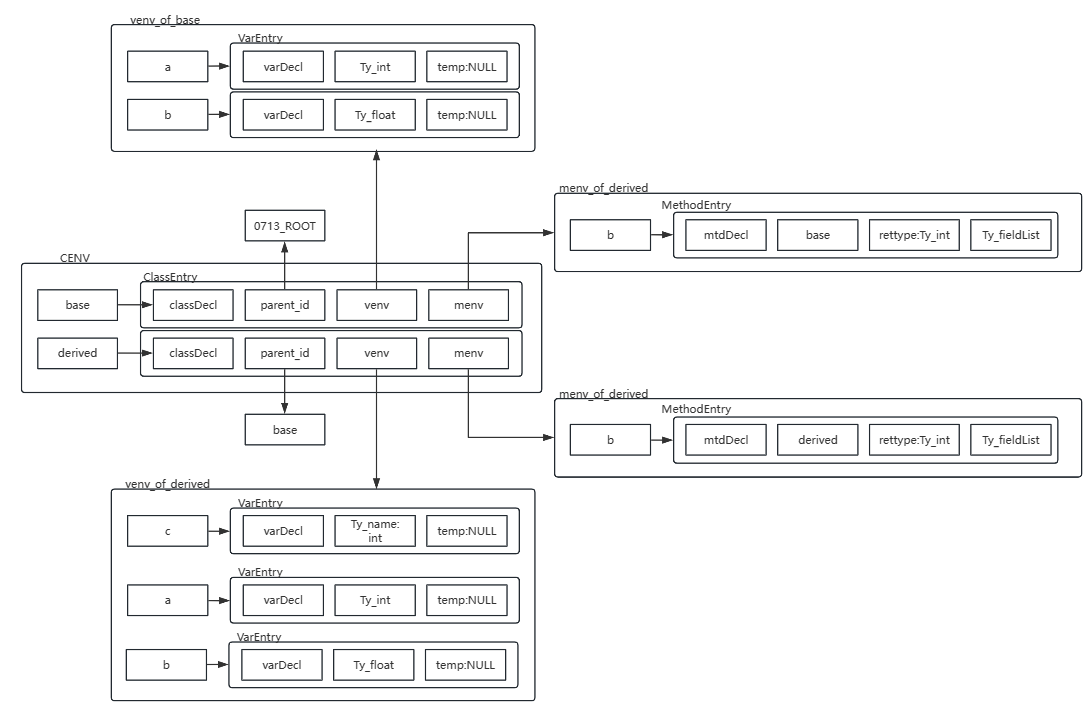
\includegraphics[width=.9\linewidth]{pics/cenv.jpg}
  \caption{样例程序的CENV结果}
  \label{fig:cenv}
\end{figure*}
其中因为base是一个基类,没有父类的类我们给它一个dummy父类,名为0713\_ROOT。同时,子类derived的venv中有继承自父类的变量a和b。

获取类环境后,我们在transA\_Classes中检查所有的、之前跳过的类型是一个类的类变量,其类型是否是一个被定义的类。然后遍历类的方法列表,调用transA\_ClassMethod检查类的每一个方法中的类型是否正确。

\subsubsection{主方法的检查过程}
主方法类型检查的入口为transA\_MainMethod。主方法的类型检查流程较为简单,基本为线性流程。首先调用transA\_VarDecList构建变量环境VENV,然后调用transA\_StmList对每一条statement进行类型检查。所用的数据结构与上方CENV的样例完全类似。

\subsubsection{类型检查的几个重要函数}
\begin{lstlisting}
static Tr_exp transA_VarDecList(FILE *out, A_varDeclList vars, S_table venv);
\end{lstlisting}
接收变量定义列表vars,输出变量环境到venv。

\begin{lstlisting}
static expty transA_Exp(FILE *out, A_exp exp, int* has_location);
\end{lstlisting}
接收一个表达式exp,返回它的类型,并将其是否有location设置到*has\_location中。

\begin{lstlisting}
static Tr_exp transA_Stm(FILE* out, A_stm stm);
\end{lstlisting}
接收一个语句stm,检查它的类型使用是否正确。

\begin{lstlisting}
static void build_menv(FILE* out, A_classDecl cls, S_table menv);
\end{lstlisting}
接收一个类定义列表cls,输出方法环境到menv。

另有一些helper functions,但不涉及到类型检查的主流程。各方法的详细实现参见src/lib/frontend/semant.c,其中有一些代码注释可以帮助理解,在此不作赘述。

\subsection{Translation to IR}
完成类型检查之后,编译器前端的处理基本就结束了,下一步是将AST转换为中间表示IR。我的实现中,将其转换为Tiger IR+,详细结构定义见文件src/include/utils/dsa/tigerirp.h。

这一步其实可以与类型检查同步进行,这也是为什么在类型检查部分的函数,都以“trans”开头来命名。具体而言,当类型检查完一条语句或者一个表达式后,不仅返回该表达式的类型(如果有),还要返回表示该语句或表达式的IR数据结构节点。因为类型检查的过程也是递归遍历整个AST,所有这个过程是可以同步进行的。

我的具体实现中,在transA\_Exp和transA\_Stm的return语句调用对应的、实现在src/lib/frontend/translate.c中的构造函数。但是为了减少semant模块和translate模块的耦合性,我们使用了一个公共的数据结构Tr\_exp作为两个模块信息传递的媒介。具体而言,semant模块生成Tr\_exp,并调用translate模块的构造函数;translate模块的构造函数根据其参数(包含Tr\_exp),将之解析转换为它期望的Tiger IR+中的数据结构节点。

translation结束之后,我们得到一个完整的Tiger IR+表示的程序,以样例程序为例,它的IR表示参见src/docs/example/example\_in\_report.3.irp文件。

\subsubsection{实现中的一些关键点}
\begin{itemize}
    \item \textbf{T\_Seq的正确使用}:由于T\_Seq默认不是以NULL结尾,并且只有一条stm时不应该使用T\_Seq,这给之前semant时,许多用到递归的地方带来了不小的影响。为了不大幅度影响总体逻辑,我实现了一个简单的sequence buffer,当翻译线性表结构的时候,首先将元素的指针存于buffer,再调用函数将这些元素组合成可能的T\_Seq,提供了可变长参数的宏Sequence()来增加可读性。这看似没有必要,但是像翻译VarDecList中可能存在声明时初始化的情况,可以提供很大的便利。sequence buffer的另一种使用方式是手动调用seqBufPush添加元素,然后使用宏SequenceFromBuffer()获得T\_Seq序列。

    \item \textbf{patchList和doPatch}:这是正确处理if语句和while语句的关键。因为在translate这两种语句中的布尔表达式时,暂时不知道其跳转的目的标签。因此我们的处理方式是将其暂时留存,利用patchList存放需要跳转到同一个标签的这些留存位置,当我们能够确定这些位置所需要填入的标签时,用doPatch进行填充。例如样例程序中,if(b.a == d.a),在翻译完b.a == d.a并解析为一个跳转的节点时,因为要调用IR中跳转结构的构造函数T\_Cjump,需要指定参数true label和false label,但此时label尚未可知,需要等到调用Tr\_IfStm翻译这条if语句时才能确定,在Tr\_IfStm函数中使用patchList和doPatch机制进行标签的填放。

    \item \textbf{检查是否处于while语句中}:维护了一个栈while\_stack,存放while语句的test标签和end标签,既可以用于continue和break的semant阶段,也方便translate阶段patch这些标签。

\end{itemize}

\subsubsection{弃用了unified object record,用offset\_env记录类成员的偏移信息}
因为unified object record会导致开辟多余的空间,在类数量多或者有几个十分庞大的类时,生成的程序对空间的利用率大大降低。为了解决这个问题,我的实现方式是:为每一个类记录一个私有的offset表。

新增了一个的全局表OFFSET\_ENV,记录类中每个成员内存位置的偏移量,从arch\_size开始(为了与null区分,表中记录时不从0开始,最后生成指令时才从0开始)。

新增了一个新的E\_enventry类型:

    \begin{lstlisting}
    E_enventry E_OffsetEntry(unsigned long long local_size, S_table local_offtbl);
    \end{lstlisting}

全局表OFFSET\_ENV存储class\_name -> local\_offtbl的映射。

每一个类的local\_offtbl中存储member\_name -> private\_offset的映射。

重要性质: 父类的所有offset全都处于前半部分,子类只在父类的offset项后面新增。

处理offset的流程如下:

    1. 在为每一个类建立venv时,同步记录和增加local\_offtbl

    2. 在为每一个类建立menv时,暂不记录method的偏移(因为可能是重写父类的方法,父类中已经记录了相应的偏移)

    3. 检查继承关系时,先继承父类的offset表,再继承var表和method表,最后再将新增的子类方法的偏移加到子类offset表的末尾(完成第2步中未记录的偏移量)

    4. 继承父类的offset表时,子类的offset表中只包含子类新增的var的偏移,为了维护上方所说的“重要性质”,将子类的表中各项的offset加上父类offset表的size(即偏移)

仍然以样例程序为例,最后得到的offset\_env结构和内容(以arch\_size=8为例)如下:
\begin{figure*}[h]
  \centering
  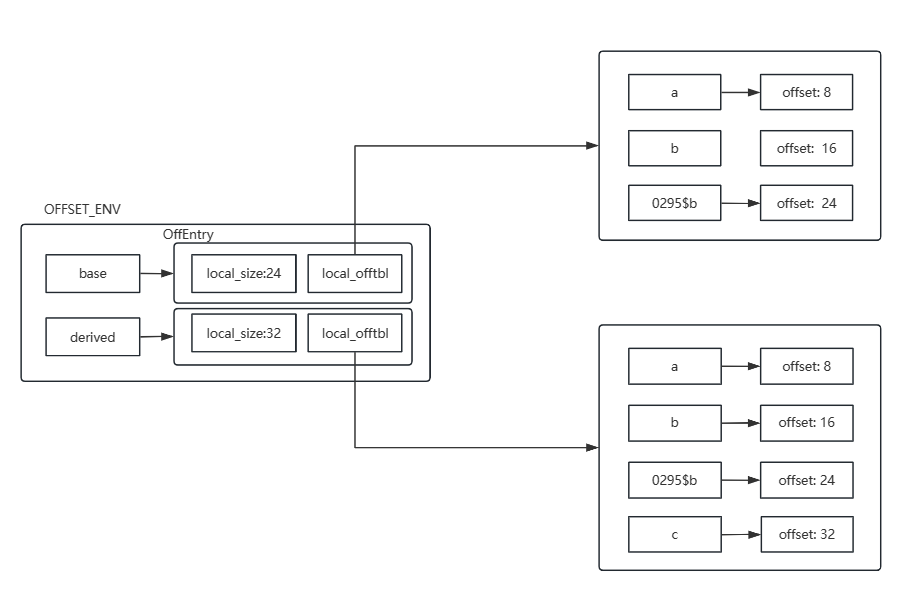
\includegraphics[width=.9\linewidth]{pics/off_env.jpg}
  \caption{样例程序的OFFSET\_ENV结果}
  \label{fig:oenv}
\end{figure*}

c是derived子类自己的类变量,因此根据“重要性质”,偏移量在所有父类变量之后。在类的方法前面加上一个0295\$,使得重名的变量和方法可以被区分。

\subsection{Canonicalization}
这是整个前端的最后一个阶段。注意到在我们使用的Tiger IR+中,有T\_Seq和T\_Eseq这类只表示结构信息的节点,它们的内容才是真正的一条条需要被执行的语句。为了去除这些不能被真正执行的节点,得到一个线性执行的语句列表,我们需要对IR进行Canonicalization。

Canonicalization主要分三步进行:第一步是linearize,得到一个线性语句列表;第二步是根据这个线性语句列表,转换为多个basic block,每一个basic block以一个标签开头,以一条跳转指令结尾;第三步是trace,将第二步得到的多个basic block重新合并为新的线性语句列表,以满足一些性质。我们的实现位于src/lib/optimizer/canon.c文件,样例程序经过Canonicalization之后的结果见src/docs/example/example\_in\_report.4.stm文件。

\subsubsection{linearize}
入口函数为:

    \begin{lstlisting}
    T_stmList C_linearize(T_stm stm);
    \end{lstlisting}

接受一个IR节点stm,调用linear函数和do\_stm函数将它线性化,返回一个链表。

linear函数递归遍历所有stm节点,如果当前节点为T\_Seq,提取其中的左右子节点,重组为线性结构。如此迭代进行,可消除所有的T\_Seq节点。

do\_stm函数主要是将一个stm节点中的T\_Eseq节点完全消除,具体做法是用一个等价的T\_Seq节点重新表示每一个T\_Eseq节点。

\subsubsection{basic block}
入口函数为:

    \begin{lstlisting}
    struct C_block C_basicBlocks(T_stmList stmList);
    \end{lstlisting}

接受第一步得到的线性语句列表stmList,输出多个basic block。

linearize的结果中,第一个块一定没有label作为开头,因此用一个新的label加到开头。使用mkBlocks函数递归提取basic block,如果一个stmList不是以label开头,加入一个新label;如果以label开头,调用next函数寻找当前basic block的结束位置。

较难理解的点主要是next函数:

    \begin{lstlisting}
    static C_stmListList next(T_stmList prevstms, T_stmList stms, Temp_label done);
    \end{lstlisting}

如果当前语句节点stms的内容为jump、cjump或return,表明达到了一个basic block的结尾,调用mkBlocks进行后续basic block块的提取。

如果直到遇到下一个basic block的label都没遇到跳转,这说明需要向上一个basic block的末尾添加一个“不必要”的跳转语句,跳转到这个label。之所以称之为不必要,是因为源程序是顺序执行,本来没必要添加这个跳转语句,但是为了满足basic block的性质而添加。

此步骤返回一个C\_block结构的数据,对于样例程序而言,结果如下图:
\begin{figure*}[h]
  \centering
  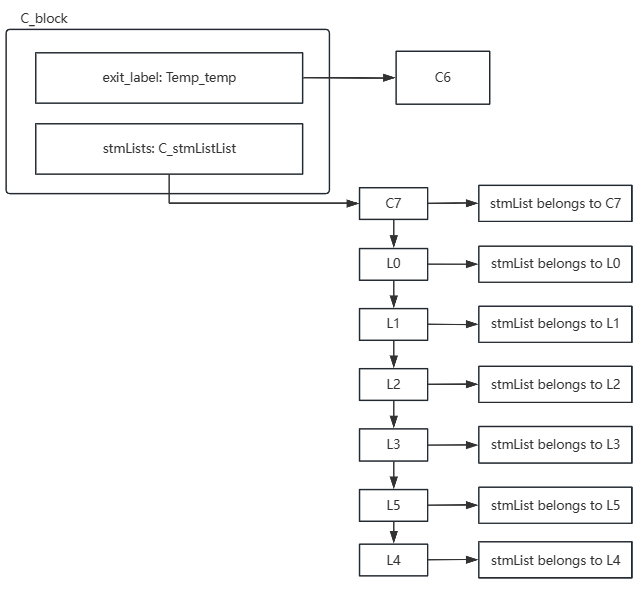
\includegraphics[width=.9\linewidth]{pics/c_block.jpg}
  \caption{样例程序的C\_block结果}
  \label{fig:cblk}
\end{figure*}

\subsubsection{trace}
trace的目的是为了让每一条cjump语句,紧跟着的下一个basic block都是它的false label,其入口函数为:

    \begin{lstlisting}
    T_stmList C_traceSchedule(struct C_block b);
    \end{lstlisting}

该函数首先构建一个表block\_env,每个表项形如“label-->stmList”,记录一个basic block的起始标签到它的语句列表首节点的映射。

然后进行trace过程。如果没有basic block,那么添加一个dummy basic block作为程序的退出点,它的内容只有一个标签和ret -1。否则如果是一个存在于block\_env中的basic block,调用trace函数使其满足性质。

trace函数中,找到当前basic block的label和最后一条语句,如果最后一条语句是jump语句,并且label存在,那么可以进行合并后去除jump语句,否则保留jump语句;如果最后一条语句是cjump,根据true label和false label是否存在,来判断紧跟着的下一个basic block到底是哪个label,如果都不存在,则修正这条cjump语句,强行让它的false label为下一个basic block。

样例程序trace之后的结果请参见:src/docs/example/example\_in\_report.4.stm中“------Canonical IR Tree------”部分

\section{Backend}
\subsection{LLVM Instruction Selection}
前端部分向我们提供了Canonicalization之后的Tiger IR+形式的中间表示,后端根据这个中间表示,生成目标平台上的汇编代码。本阶段进行Tiger IR+到LLVMIR的转换。LLVMIR不仅可作为一种中间表示,也可以在LLVM的环境下运行。

LLVM Instruction Selection的具体实现在src/lib/backend/llvm/llvmgen.c文件。

保存指令选择结果的数据结构为AS\_instr,定义在src/include/utils/dsa/assem.h文件中。共有三种kind,其中I\_OPER最为常用,包含字符串形式的汇编指令assem、使用到的源temps列表dst和目的temps列表src、跳转地点jumps。assem只是一个格式字符串,会在src/lib/utils/dsa/assem.c文件中定义的format函数里完成相应的格式替换,“`di”被替换为dst中第i个temp的name,“`si”被替换为src中第i个temp的name,“`ji”被替换为jumps中第i个label的name(这里i为0从开始的整数)。

以样例程序derived\$b函数的Canonical IR Tree为例,它将被转化为如图\ref{fig:asm}所示的数据结构:

\begin{figure*}[h]
  \centering
  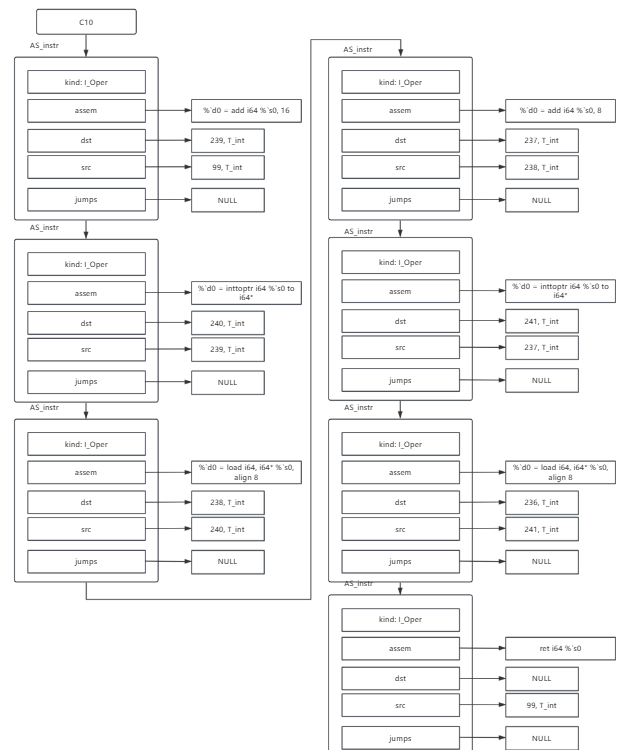
\includegraphics[width=.6\linewidth]{pics/assem.jpg}
  \caption{样例程序derived\$b函数的llvm instruction selection结果}
  \label{fig:asm}
\end{figure*}

经过格式化并打印后的结果为:

\begin{lstlisting}
    C10:
    %r239 = add i64 %r99, 16
    %r240 = inttoptr i64 %r239 to i64*
    %r238 = load i64, i64* %r240, align 8
    %r237 = add i64 %r238, 8
    %r241 = inttoptr i64 %r237 to i64*
    %r236 = load i64, i64* %r241, align 8
    ret i64 %r236
\end{lstlisting}

LLVM指令选择的过程遍历Tiger IR+中的T\_funcDeclList,对于每一个T\_funcDecl,调用llvmprolog函数获取llvm代码中的函数定义,例如样例中derived类的b函数,返回的数据结构携带的指令为“define i64 @derived\$b(i64 \%r99)\{”;调用llvmepilog获取llvm代码中的函数结束部分,例如样例的main函数,返回的数据结构携带的指令为“\}”。

重点在于函数语句的指令选择,入口函数为:

    \begin{lstlisting}
    AS_instrList llvmbody(T_stmList stmList);
    \end{lstlisting}

该函数遍历所有stm,调用munchStm函数进行指令选择。其中munchStm根据stm的类型kind,输出等价的llvm指令来完成一条T\_stm。

另有两个函数munchExp和munchMove。

munchExp是用于获取表达式的值,例如一个exp为T\_CONST,那么将它的值move到一个temp中,并返回这个temp。即输入一个exp,munchExp返回存有这个exp的值的temp。

munchMove是为了优化对T\_Move的指令选择。因为如果在获取需要move的值的时候,直接把目的temp传递给munchExp使用的话,就可以减少一条“move temp1, temp2”形式的指令。

对于样例程序指令选择并格式化打印输出后的结果,参见src/docs/example/example\_in\_report.5.ins文件。

\subsection{Liveness Analysis}
Liveness Analysis是为了分析数据的流动和活跃范围,以便我们获取丰富的数据流信息和temp活跃情况。

活跃分析基于图进行,因此简要介绍一下我们使用的图结构(定义在src/include/utils/dsa/graph.h中)。每个图节点为G\_node,其中mygraph成员为其所属图、mykey成员为其在图上的标号、succs为前驱节点、preds为后继节点、info可以是任何与之关联的信息。每个图G\_graph,其中nodecount表示节点数、mynodes表示图上的节点列表,mylast表示最后一个加入到图中的节点。针对图操作的函数参见代码注释。

\subsubsection{flow graph}
活跃分析是基于流图进行的,因此我们首先需要根据指令选择之后得到的指令序列,构建它的流图。流图中每一个节点对应一条指令,有向边表示跳转关系。flow graph相关的代码实现位于src/lib/optimizer/flowgraph.c文件。

构建流图的入口函数为:

    \begin{lstlisting}
    G_graph FG_AssemFlowGraph(AS_instrList il);
    \end{lstlisting}

该函数遍历所有assem指令,生成对应的图节点并维护前后跳转关系,同时维护了一个表,用于存放每个节点对应的def的temp和use的temp列表,后续通过FG\_def和FG\_use获取这些信息。

\subsubsection{liveness}
有了流图之后,我们根据公式:
\begin{figure*}[h]
  \centering
  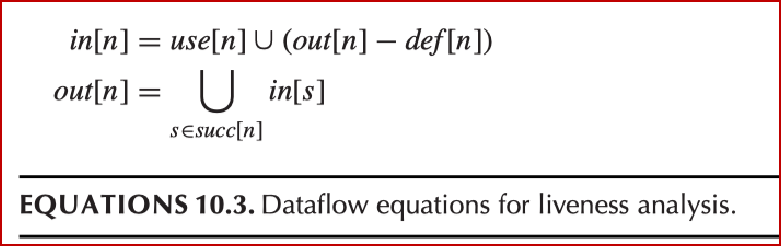
\includegraphics[width=.9\linewidth]{pics/liveness_theory.png}
  \label{fig:liv_theory}
\end{figure*}

不断迭代,直到达到不动点,即为liveness的结果。

该过程的相关实现位于src/lib/optimizer/liveness.c文件,入口函数为:

    \begin{lstlisting}
    G_nodeList Liveness(G_nodeList nodes);
    \end{lstlisting}

其中参数nodes为flow graph的节点,该函数不断循环调用LivenessIteration,根据是否产生变化(即是否达到不动点)来决定是否继续循环。LivenessIteration是对上述公式的一次迭代,并保存或更新信息到表InOutTable,返回这轮迭代是否导致liveness结果产生变化。

liveness的结果通过FG\_In和FG\_Out访问,本质就是查InOutTable这个表。

对于样例程序的liveness结果,参见src/docs/example/example\_in\_report.5.ins文件。

\subsection{Static Single Assignment}
静态单赋值(Static Single Assignment,简写为SSA)是一种指令序列的形式,其满足每个temp只被定义一次,可被使用多次。

在这一阶段,我们将可能不满足SSA形式的指令序列转换为满足SSA形式的指令序列。转换为SSA形式的具体实现位于src/lib/optimizer/ssa.c文件,入口函数为:

    \begin{lstlisting}
    AS_instrList AS_instrList_to_SSA(AS_instrList bodyil, G_nodeList lg, G_nodeList bg);
    \end{lstlisting}

其中bodyil为函数体指令序列,lg为具有liveness信息的图节点,bg为control flow graph。

\subsubsection{control flow graph}
一个basic block内部是线性的,没有跳转,因此没必要直接对它内部的流图节点计算dominators。我们只需要计算各个basic block直接的dominate情况,因此我们构建新的图,控制流图(control flow graph,cfg)。
控制流图类似于流图,只是图上每个节点代表一个AS\_Block形式的basic block,而非一条指令。
构建控制流图的入口函数为:

    \begin{lstlisting}
    G_nodeList Create_bg(AS_blockList bl);
    \end{lstlisting}

该函数也是遍历所有AS\_block,根据每个basic block最后一句指令的跳转关系,来添加有向边到图上的节点。

样例程序main函数的的cfg结果如下(括号中为当前节点,冒号右侧为它的后继):

\begin{lstlisting}
    C7 (0): 1 5 
    L1 (1): 2 
    L2 (2): 3 
    L3 (3): 4 6 
    L4 (4): 
    L0 (5): 2 
    L5 (6): 3 
\end{lstlisting}

化成图的形式为:

\begin{figure*}[h]
  \centering
  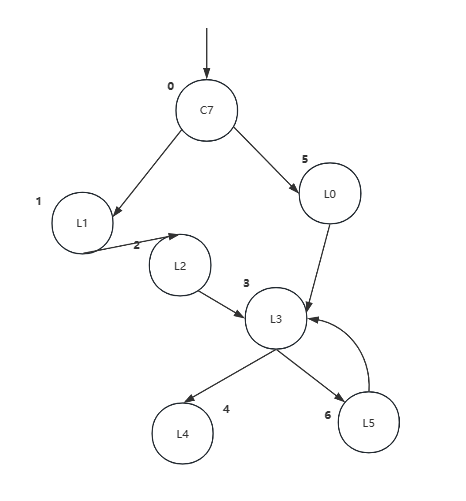
\includegraphics[width=.5\linewidth]{pics/cfg.jpg}
  \label{fig:cfg}
\end{figure*}

\subsubsection{steps}
\textbf{1.计算dominators和immediate dominator}

计算公式为:
\begin{figure*}[h]
  \centering
  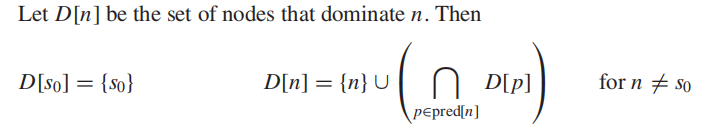
\includegraphics[width=.9\linewidth]{pics/dominators.jpg}
  \label{fig:dom_theory}
\end{figure*}

此步骤先由

    \begin{lstlisting}
    static void compute_dominators(G_table dominators);
    \end{lstlisting}
    
计算出所有节点的dominators表。dominators表,初始化为“node->all nodes”的形式(除了startnode起始节点外,所有的node一开始初始化为dominate所有节点,startnode只dominate它自己)。其中node是control flow graph上的图节点。该函数依据公式不断迭代,直到达到不动点,代码与公式的对应关系参见代码注释。函数结束后,dominators表记录了每个节点(key)被哪些节点(value)所dominate。

然后调用retrive\_immediate\_dominator函数构建dominator tree,以邻接表的形式存放到表格idom中,idom中记录了每个节点(key)的直接dominator(value)。

对于样例程序,此步的结果如下:

\begin{lstlisting}
    (1): 0
    (2): 0
    (3): 2
    (4): 3
    (5): 0
    (6): 3
\end{lstlisting}

对应的dominator tree为:

\begin{figure*}[h]
  \centering
  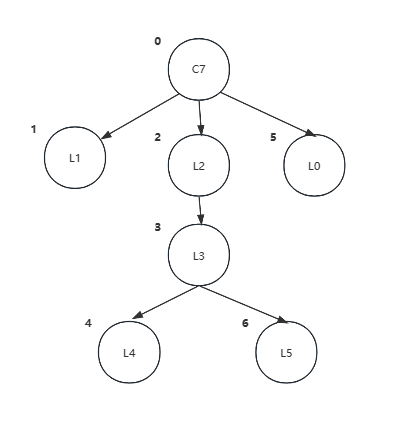
\includegraphics[width=.74\linewidth]{pics/idom.jpg}
  \label{fig:idom}
\end{figure*}

\textbf{2.计算dominance frontier}

算法为:
\begin{figure*}[h]
  \centering
  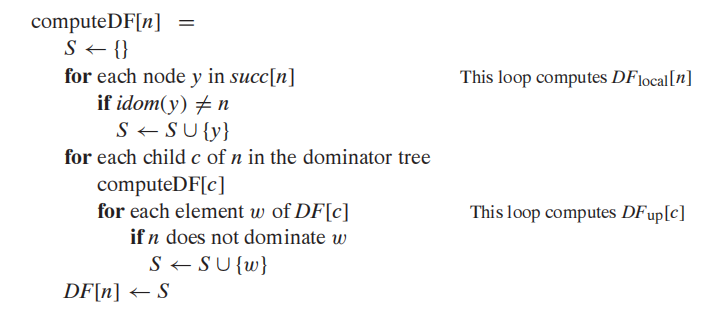
\includegraphics[width=.6\linewidth]{pics/df.jpg}
  \label{fig:df_theory}
\end{figure*}

该算法有一小错误: "if n does not dominate w" 应为 "if n does not strictly dominate w"

我的实现位于compute\_dominance\_frontier\_impl函数,compute\_dominance\_frontier函数只是一个入口。我的实现与上述伪代码表示的算法的对应关系参见代码注释,在此不作赘述。

对于样例程序的main函数,此步结果为:

\begin{lstlisting}
    (0):
    (5): 2
    (2):
    (3): 3
    (6): 3
    (4):
    (1): 2
\end{lstlisting}

\textbf{3.插入phi函数}

算法为:
\begin{figure*}[h]
  \centering
  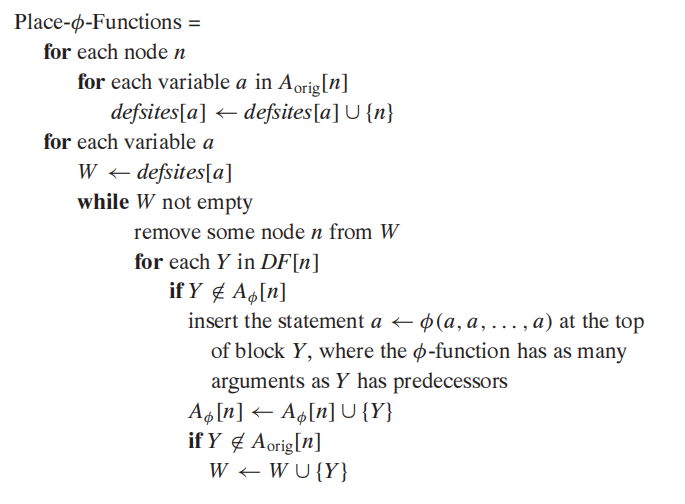
\includegraphics[width=.7\linewidth]{pics/phi.jpg}
  \label{fig:phi_theory}
\end{figure*}

对于最内层的:

\begin{lstlisting}
    for each Y in DF[n]:
    if Y not in A_phi[n]:
        insert
        A_phi[n] |= Y
        if Y not in A_orig[n]:
            w |= Y
\end{lstlisting}

应为:

\begin{lstlisting}
    for each Y in DF[n]:
    if a not in A_phi[Y]:
        insert
        A_phi[Y] |= a
        if a not in A_orig[Y] and a in live-in of Y:
            w |= Y
\end{lstlisting}

在我的实现中首先初始化表格结构记录信息,包括记录“temp->defsites”的表格、记录算法中$A_{\phi}$与$A_{orig}$的表格、记录每个cfg节点对应的live-in和live-out的表格。初始化完毕这些基本信息之后,根据上述伪代码编程实现即可。我的实现与上述算法的对应关系参见代码注释,插入phi函数时有多少个前驱结点就需要插入多少个phi函数的参数,为后续的重命名预留空间。

\textbf{4.重命名temp}

算法为:
\begin{figure*}[h]
  \centering
  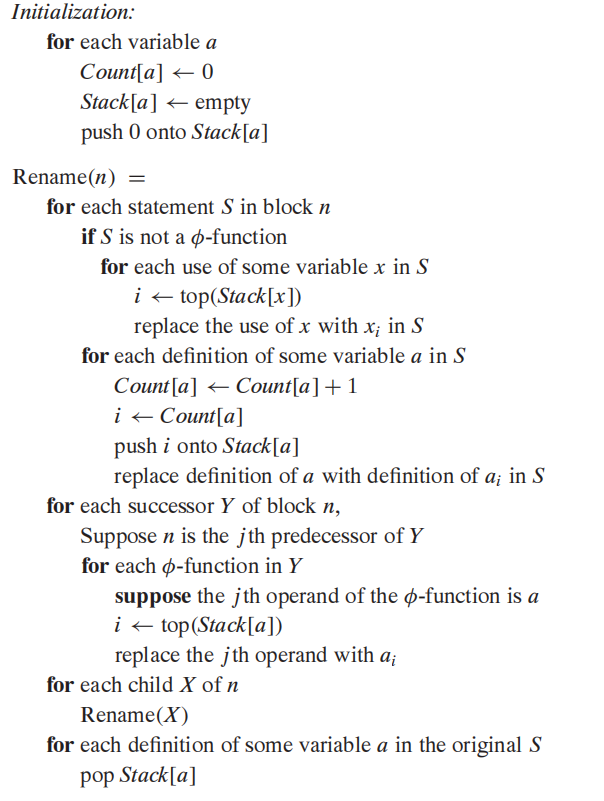
\includegraphics[width=.6\linewidth]{pics/rename.jpg}
  \label{fig:rename_theory}
\end{figure*}

在具体实现上,我使用表来实现了算法中的stack。基于底层的TAB\_table,实现了Temp\_stack,存放“temp->renamed temp”的映射。并支持beginScope机制和endScope机制,插入一个特殊的temp(其num为-1)来标识Scope的开始,控制重命名的有效域。

该步骤的入口函数为rename\_temps,初始化Temp\_stack为“temp->temp”(即未重命名)的状态,然后调用rename\_temps\_impl函数。

rename\_temps\_impl函数从dominator tree的根节点开始递归遍历。函数开始前先beginScope。然后对于当前重命名的basic block(对应节点为rename\_temps\_impl函数的第一个参数n)中的所有非label指令,如果不是phi函数,那么对它use中的temps重命名;不论是不是phi函数,对它def中的temps重命名为一个新的temp并记录到stack中。接着按照上述算法,重命名它的后继节点中可能存在的phi函数中的变量。最后递归遍历后继节点,退出前endScope防止子节点的重命名影响其它子节点。

\subsection{RPi Instruction Selection}
该阶段也属于指令选择(Instruction Selection),本质与LLVM Instruction Selection没有区别。区别在于LLVM Instruction Selection的输入为Tiger IR+树,而RPi Instruction Selection的输入为LLVM指令序列构成的basic block,因此RPi Instruction Selection需要大量识别和处理字符串。具体实现位于src/lib/backend/arm/armgen.c文件。

在正式进行指令选择之前,需要去除phi函数,因为没有真实的arm指令可以实现phi函数的功能。我们通过在有phi函数的地方,找到这个basic block的所有前驱节点,在它的跳转指令之前添加对应的move指令,这样就可以用多条指令,实现phi函数的效果。

然后类似于llvmbody,我们根据不同的llvm指令,选择与之对应的arm指令即可。一些关键点在于:
\begin{itemize}
    \item \textbf{立即数处理}:所有立即数都使用两次ldr指令加载它的类模式到寄存器,以防止它是不合法的立即数。

    \item \textbf{简单的常量折叠}:有大部分的代码用于识别LLVM指令中两个操作数的类型组合方式(register-register, register-immediate, immediate-register, immediate-immediate),并在immediate-immediate的情况下进行编译时计算。

    \item \textbf{函数调用的传参}:我们的函数规定最多有三个参数,加上this参数,最多需要四个寄存器来传递参数。用r0-r3传递int型参数,用s0-s3传递float型参数。为了提取函数调用的参数及其类型,我在src/lib/backend/arm/armgen.c中新定义了数据结构Arg,和ArgList,作为extract\_args函数的输出和对call指令进行rpi指令选择时的输入。每个Arg结构的成员为:tp记录该Arg是T\_int还是T\_float、isConst记录是立即数还是temp、联合体u用于获取对应的数据。

\textbf{需要注意的是},在指令选择这一阶段,我并未对栈帧、caller-save和callee-save寄存器进行处理,而是把这些工作留到了最后的寄存器分配阶段。但是如果非要生成具有一定栈帧结构的指令,只需将入口函数AS\_instrList\_to\_arm的参数save\_all\_callee设置为TRUE即可,为FALSE是不具有栈帧结构的。

\end{itemize}

\subsection{Register Allocation}
这一阶段将rpi指令转换为可执行的形式。因为对于真实的机器而言,不可能有无限个temp(即无限个寄存器)供使用,因此我们需要将上一阶段生成的指令中的temp,映射为真实的寄存器。这一阶段的实现位于src/lib/backend/arm/regalloc.c文件。

我实现寄存器分配的算法是simplify and spill。在我的实现中,r0-r10为可用整型寄存器,其中r0-r3为caller-save,r4-r7为callee-save,r8-r10专门用于spill;s0-s31为可用浮点寄存器,其中s0-s15为caller-save,s16-s28为callee-save,s29-s31专门用于spill。

\subsubsection{Interference Graph}
我们的寄存器分配依赖于Interference Graph,该图是无向图,记录了各个temp之间的冲突关系,即如果两个temp之间存在一条边,则这两个temp不能被分配到同一个寄存器。因此,寄存器分配等价于对Interference Graph进行图着色问题。Interference Graph的图节点关联一个temp,构建Interference Graph的依据为:
\begin{figure*}[h]
  \centering
  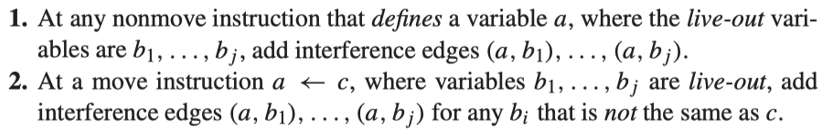
\includegraphics[width=.6\linewidth]{pics/ig_threory.jpg}
  \label{fig:ig_theory}
\end{figure*}

因此构建Interference Graph前需要重新对rpi指令进行活跃性分析,利用活跃性分析的结果,调用Create\_ig函数构建Interference Graph。过程十分简单,遍历所有的flowgraph node,满足

\begin{lstlisting}
    (!(is_m && tl2->head == use->head)) && (tl2->head != tl1->head) 
    && (tl2->head->type == tl1->head->type)
\end{lstlisting}
条件的就添加一条边(node(tl1->head), node(tl2->head))到图中。第一个条件子句是对move指令的特殊处理,第二和第三个条件子句要求没有指向自己的环,并且分离了整型和浮点型。

\subsubsection{implementation details}
以样例程序中的main函数为例,由于main函数涉及到的temp过多,因此下方展示的结果只挑选了其中具有代表性的几个temp来说明我的实现方法。

寄存器分配的入口函数regalloc中:

首先调用simplify\_and\_spill函数,该函数接收Interference Graph,对于所有可用寄存器,设有k个,不断删除Interference Graph上节点度小于k的节点并入栈标记为color;不能删除之后任选一个非预着色的节点删除并入栈,标记为spill,直到所有非预着色的节点被删除。删除的过程中记录节点删除时的前驱后继。注意区分temp的类型,整型的temp和浮点型的temp使用不同数量的寄存器。这些标记信息存放于栈simplify中。对于样例程序的main函数而言,少数结果如下:

    \begin{lstlisting}
    r252: color
    r210: spill
    r220: spill
    \end{lstlisting}

然后调用color\_and\_actual\_spill,该函数根据simplify\_and\_spill产生的栈simplify,反向弹出栈中的temp并根据记录的删除时的前驱后继节点回复图的拓扑结构。如果标记为color,随便分配一个可用寄存器,并记录到表color中。如果标记为spill,需要先判断它目前的邻居是否用完了所有k个寄存器,如果没用完,也可以分配没用到的一个寄存器给它并记录到表color中;否则需要进行actual spill,在栈上分配一块空间(4字节)给这个temp,并记录它的offset到表spill中。对于样例程序中main函数,两个表的结果如下:

color表的结果(此前被标记为spill的r210没有发生actual spill):
    \begin{lstlisting}
    r252->r1
    r210->r1
    \end{lstlisting}

spill表的完整结果(包含了r220):
    \begin{lstlisting}
    r226 actual spilled to fake offset 32
    r220 actual spilled to fake offset 28
    r195 actual spilled to fake offset 24
    r193 actual spilled to fake offset 20
    r182 actual spilled to fake offset 16
    r181 actual spilled to fake offset 12
    r180 actual spilled to fake offset 8
    r179 actual spilled to fake offset 4
    \end{lstlisting}

构建完color和spill两个表之后,我们就可以对原始rpi指令中用到的temp进行替换。对于color中的temp直接替换即可,对于spill中的temp,使用哪个寄存器,取决于它出现在一条rpi指令中从左到右的位置。因为一条rpi指令最多用到三个寄存器,因此预留3个寄存器专门用于spill。在每一个发生actual spill的temp被def的指令,加上str指令将其保存到栈上对应的offset处;在每一个发生actual spill的temp被use的指令之前,加上ldr指令,取出栈上对应offset处的数据。需要注意的是这里的offset相对于fp而言向下增长,且暂时没有考虑栈帧大小,所以这是暂时的offset。

对于上述例子中发生actual spill的r220,def它的指令为:

    \begin{lstlisting}
    mov r220, r195
    \end{lstlisting}

actual spill之后变为(因为r195也进行了actual spill,且位于这条指令从左到右第2个寄存器,所以用r8,r9,r10中的第2个寄存器r9来进行spill):

    \begin{lstlisting}
    ldr r9, [fp, #24]
    mov r8, r9
    str r8, [fp, #28]
    \end{lstlisting}

最后调用函数build\_frame构建栈帧。在入口保存栈帧和必要的callee-save寄存器,在所有ret指令之前加入弹出的指令。为什么不需要保存caller-save寄存器呢?这是因为我们在进行interference graph的计算前,将每一个函数调用指令的def列表中,加入了所有caller-save寄存器。这样处理之后,在每一条函数调用指令之后的指令中用到的temp,永远会与caller-save寄存器这些预着色节点发生冲突,导致这些函数调用指令之后的指令中用到的temp只能被分配到callee-save寄存器,因此也就无需要保存caller-save寄存器了。处理完栈帧之后需要处理发生actual spill的temp对应的offset,将这些offset加上num\_used\_callee * ARCH\_SIZE并取负(向下增长)即得到真正的相对于fp的offset。如果此时栈没有8字节对齐,需要将栈调整到8字节对齐,以解决调用putfloat时产生的错误。

因为一共保存了r4-r9,共ARCH\_SIZE * 6 = 24字节,上述例子现在变为:

    \begin{lstlisting}
    ldr r9, [fp, #-48]
    mov r8, r9
    str r8, [fp, #-52]
    \end{lstlisting}

\section{Conclusion}
以上便是对一个编译器最基本的流程和我对应实现的阐述。关于如何使用我的代码构建出所述编译器并使用,首先需要简单介绍一下代码目录的组织与管理。项目主要使用CMake和Makefile进行管理,src是编译器的源代码目录,test用于存放测试所用的.fmj源文件。

在代码的根目录下,根据以下指令进行构建和使用:
\begin{itemize}
    \item \textbf{make build}:使用cmake与makefile对项目进行编译链接,生成编译器的可执行文件main到目录build。

    \item \textbf{make compile}:利用生成的编译器main,将test文件夹中的所有.fmj文件进行编译,并产生对应的中间输出,其中.6.ssa文件是可在llvm环境下运行的指令文件,.8.s文件是最终的可在qemu-arm上运行的汇编代码。
    
    \item \textbf{make run-llvm}:重新编译,并使用llvm的环境运行ssa形式的llvm指令文件。

    \item \textbf{make run-rpi}:重新编译,并使用qemu-arm环境运行汇编.8.s汇编文件之后的机器代码。
\end{itemize}
也可以直接运行main函数,其提供.fmj文件的路径,与make compile产生相同的结果。

总结而言,通过本学期的课程,我掌握了基本的编译技术及其实现方式,也有思考将课堂所学的编译知识应用到其他领域的场景,例如利用寄存器分配的思想来优化深度学习训练框架中的显存分配与使用(将显存分块视为一个个寄存器,计算图上的tensor节点视为一个个temp)。这是一门让我受益匪浅的课程,不仅锻炼了我的代码实践能力,还让我掌握了更多样地分析计算机世界中问题的思想与方法。

感谢参阅!

\end{document}
